\title{A load-aware scheduler for large-scale neural network autotuning}
\author{Dominik Stiller}
\date{September 2019}

\documentclass{scrreprt}


%----------------------------------------------------------------------------
% Package Includes
%----------------------------------------------------------------------------
\usepackage[USenglish]{babel}
\usepackage[T1]{fontenc}
\usepackage[utf8]{inputenc}
\usepackage{lmodern}

\usepackage{tocloft}
\usepackage{chngcntr}
\usepackage{amsmath}
\usepackage{mathtools}
\usepackage{interval}
\usepackage{graphicx}
\usepackage[hidelinks]{hyperref}
\usepackage{geometry}
\usepackage{textcomp}
\usepackage{siunitx}
\usepackage{setspace}
\usepackage{array}
\usepackage[outputdir=build]{minted}
\usepackage{tabularx}
\usepackage{makecell}
\usepackage{csquotes}
\usepackage[toc,nonumberlist,acronym,nopostdot]{glossaries}
\usepackage[
	backend=biber,
	bibwarn=true,
	bibencoding=utf8,
	sortlocale=en_US,
	urldate=long,
	style=ieee
]{biblatex}
\usepackage[activate={true,nocompatibility},final,tracking=true,kerning=true,spacing=true,factor=1100,stretch=10,shrink=10]{microtype}


%----------------------------------------------------------------------------
% Package Config
%----------------------------------------------------------------------------

% KOMA-Script
\KOMAoptions{
	pagesize=pdftex,
	twoside=false,		% Einseitiger Druck.
	parskip=half,		% Halbe Zeile Abstand zwischen Absätzen.
	headheight = 12pt,	% Höhe der Kopfzeile
	headsepline,		% Linie nach Kopfzeile.
	footsepline,		% Linie vor Fusszeile.
	footheight = 16pt,	% Höhe der Fusszeile
	abstract=true,		% Abstract Überschriften
	DIV=calc,			% Satzspiegel berechnen
	%BCOR=8mm,			% Bindekorrektur links: 8mm
	headinclude=false,	% Kopfzeile nicht in den Satzspiegel einbeziehen
	footinclude=false,	% Fußzeile nicht in den Satzspiegel einbeziehen
	listof=totoc,		% Abbildungs-/ Tabellenverzeichnis im Inhaltsverzeichnis darstellen
	toc=bibliography	% Literaturverzeichnis im Inhaltsverzeichnis darstellen
}
\clubpenalty = 10000 % schließt Seitenumbruch nach der ersten Zeile eines neuen Absatzes aus
\widowpenalty = 10000 % schließt die letzte Zeile eines Absatzes steht auf einer neuen Seite aus
\displaywidowpenalty=10000

% graphicx
\graphicspath{ {./images/} }

% biblatex
\addbibresource{misc/references.bib}

% Microtype
% http://www.khirevich.com/latex/micrsotype/
\SetProtrusion{encoding={*},family={bch},series={*},size={6,7}}
			     {1={ ,750},2={ ,500},3={ ,500},4={ ,500},5={ ,500},
	             6={ ,500},7={ ,600},8={ ,500},9={ ,500},0={ ,500}}
\SetExtraKerning[unit=space]
   				{encoding={*}, family={bch}, series={*}, size={footnotesize,small,normalsize}}
				{\textendash={400,400}, % en-dash, add more space around it
	               "28={ ,150}, % left bracket, add space from right
	               "29={150, }, % right bracket, add space from left
					\textquotedblleft={ ,150}, % left quotation mark, space from right
					\textquotedblright={150, }} % right quotation mark, space from left
\SetExtraKerning[unit=space]
				{encoding={*}, family={qhv}, series={b}, size={large,Large}}
				{1={-200,-200}, \textendash={400,400}}
\SetTracking{encoding={*}, shape=sc}{40}
\microtypecontext{spacing=nonfrench}

% glossary
\renewcommand*{\glsgroupskip}{}

% chngcntr
\counterwithout{figure}{chapter}
\counterwithout{table}{chapter}
\counterwithout{equation}{chapter}

% minted
\usemintedstyle{friendly}
\newminted{python}{
	mathescape,
	linenos,
	numbersep=5pt,
	frame=lines,
	framesep=2mm
}
\newmintinline{python}{}

% amsmath
\DeclareMathOperator*{\argmax}{arg\,max}
% https://tex.stackexchange.com/a/43009
\DeclarePairedDelimiter\abs{\lvert}{\rvert}
\makeatletter
\let\oldabs\abs
\def\abs{\@ifstar{\oldabs}{\oldabs*}}
\makeatother


%----------------------------------------------------------------------------
% Styling
%----------------------------------------------------------------------------

% Page
\geometry{margin=2.5cm, foot=1cm}

% Font
\KOMAoptions{fontsize=12pt}
\DeclareMathSizes{12pt}{12pt}{15pt}{10pt}
\setkomafont{title}{\Huge\textbf}
\onehalfspacing

% Table of Contents
\setcounter{tocdepth}{1}


%----------------------------------------------------------------------------
% Custom Commands
%----------------------------------------------------------------------------

\newcommand*{\vcenteredhbox}[1]{
	\begingroup
	\setbox0=\hbox{#1}\parbox{\wd0}{\box0}
	\endgroup
}

\newcommand{\multilinecell}[2][c]{%
	\begin{tabular}
		[#1]{@{}l@{}}#2
	\end{tabular}
}


\makeglossaries
\newglossaryentry{machine learning}{
	name={ml},
	description={using computers}
}

\newacronym{cv}{CV}{computer vision}
\newacronym{ml}{ML}{machine learning}
\newacronym{ann}{ANN}{artificial neural network}
\newacronym{cnn}{CNN}{convolutional neural network}
\newacronym{gpu}{GPU}{graphics processing unit}

\begin{document}
	\pagenumbering{Roman}
	\pagestyle{empty}
	\makeatletter
	\begin{titlepage}
		\vcenteredhbox{
\includegraphics[height=2cm]{logo_hpe.png}}
\hfill
\vcenteredhbox{
\includegraphics[height=2cm]{logo_dhbw.png}}

\vfill
\begin{center}
	\rule{\textwidth}{1pt}
	{
		\Huge
		\bfseries
		A load-aware scheduler \\ for large-scale \\ neural network autotuning
		\par
	}
	\vspace{-0.2cm} 
	\rule{\textwidth}{1pt}

	\vfill

	\textsc{Project Thesis II / T2000}
	
	\vfill

	for the study program \\ \textbf{Computer Science}
	
	at the \\ \textbf{Baden-Wuerttemberg Cooperative State University Stuttgart}
	
	by \\ \textbf{\@author}
\end{center}

\vfill

\begin{tabbing}
	mmmmmmmmmmmmmmmmmmmmmmmmmm				\= \kill
	\textbf{Date}      						\> \@date \\
	\textbf{Project Period} 				\> 18 Weeks \\
	\textbf{Matriculation Number, Course}  	\> 4369179, TINF17A \\
	\textbf{Company}                        \> Hewlett Packard Enterprise \\
	\textbf{Corporate Supervisor}           \> Junguk Cho \\
	\textbf{University Supervisor}          \> Prof. Dr. Bernd Schwinn
\end{tabbing}

	\end{titlepage}
	
	\section*{Declaration of Authorship}
	I hereby declare that the thesis submitted with the title \textit{\@title} is my own unaided work. All direct or indirect sources used are acknowledged as references.

Neither this nor a similar work has been presented to an examination committee or published.

\vspace{4em}

Sindelfingen
\hspace{1.3cm}
September 12, 2019
\vspace{-0.4cm}
\\
\rule{15cm}{0.4pt}\\
Place
\hspace{2.5cm}
Date
\hspace{4.5cm}
\@author
	\makeatother

	\begin{abstract}
		Real-time computer vision applications with deep learning-based inference require hardware-specific optimization to meet stringent performance requirements. However, this approach requires vendor-specific libraries developed by experts for some particular hardware, limiting the set of supported devices and hindering innovation. The deep learning compiler stack TVM is developed to address these problems. TVM generates the optimal low-level implementation for a certain target device based on a high-level input model using machine learning in a process called autotuning.

In this paper, we first explore the capabilities and limitations of TVM's autotuning implementation. Then, we develop a scheduler to orchestrate multiple, parallel autotuning jobs on shared computation resources such as CPUs and GPUs, allowing us to minimize resource idle time and job interference. Finally, we reflect our design choices and compare the efficiency of our approach with the default, scheduler-less design.
	\end{abstract}

	\setlength{\cftbeforetoctitleskip}{0em}
	\begin{spacing}{1.15}
	   \tableofcontents
	\end{spacing}
	\clearpage
	\thispagestyle{empty}
	
	\pagestyle{plain}
	
	%----------------------------------------------------------------------------
	% Preface
	%----------------------------------------------------------------------------
	\printacronyms
	\clearpage
	
	\addcontentsline{toc}{chapter}{\listfigurename}
	\listoffigures
	\clearpage
	\addcontentsline{toc}{chapter}{\listtablename}
	\listoftables
	\renewcommand\listoflistingscaption{List of Source Codes}
	\listoflistings
	\clearpage
	
	\pagenumbering{arabic}
	
	\pagestyle{headings}
	
	\addtocontents{toc}{\protect\thispagestyle{empty}}
	\obeylines
	%----------------------------------------------------------------------------
	% Content
	%----------------------------------------------------------------------------
	\chapter{Introduction}
	In recent years, \gls{ai} has garnered tremendous success, revolutionizing the way we work and accelerating economic growth. It has the potential to increase growth rates of industries such as manufacturing and financial services by 2.1 and 1.9 percentage points respectively~\cite[p.~17]{Statista.2019}. Especially \gls{dl}, a subfield of \gls{ai}, has made vast improvements and is the prime method of modern \gls{ai}. In the future, \gls{ai} will be applied to even more areas, where non-expert users want to benefit from \gls{ai} without the technical complexity introduced by development and deployment of \gls{ai} applications. This is facilitated by platforms such as BlueData and Qubole, which automate infrastructure setup and provide user-friendly interfaces to make \gls{ai} and \gls{ai} more accessible. 

\section{Problem}
More and more applications like industrial monitoring or autonomous driving require real-time performance, most of them powered by \gls{dl}. Specialized accelerator hardware such as \glspl{gpu} or FPGAs are employed to speed up the computation-intensive inference. However, the model itself needs device-specific, low-level optimizations to harness the accelerator's full potential. Currently, these optimizations are manually developed by the device vendor who have deep knowledge of their hardware. \gls{dl} researchers, who want to experiment with new model types and high-level optimizations, are forced to wait until low-level implementations are supported by vendor libraries. Additionally, it causes vendor lock-in.

Automated performance optimization, called autotuning, creates low-level optimizations without the need for human experts in a vendor-agnostic way. This fosters innovation and helps meet increasing performance demands for a growing variety of models and accelerator devices. While autotuning is already employed, it has not yet reached widespread use, partially because it is still inconvenient to use. Offering autotuning as-a-Service can make it accessible for a larger audience to facilitate real-time \gls{dl} applications, but requires support for large-scale autotuning. However, inefficiencies in the autotuning process prohibit efficient scaling and, in turn, implementation of an Autotuning as a Service platform. To the best of our knowledge, there is no existing solution for scaling autotuning.

\section{Scope}
In this thesis, we design and create a prototypical implementation of a load-aware scheduler to enable large-scale autotuning. This scheduler controls multiple autotuning jobs that share computation resources to overcome the inefficiencies of current autotuning. We show that controlling the execution of multiple jobs by a load-aware scheduler makes large-scale autotuning more efficient in terms of
\begin{itemize}
	\item autotuning completion time,
	\item resulting inference performance, and
	\item hardware requirements.
\end{itemize}

First, we discuss manual and automated performance optimization before comparing two frameworks for autotuning (Chapter \ref{sec:background}). Next, we will develop a framework to examine capabilities and limitations of autotuning in different scenarios. This will allows us to find capabilities and limitations which we can leverage to scale autotuning (Chapter \ref{sec:using-tvm}). We will design and implement our scheduler which is used in our proposed reference architecture for Autotuning as a Service (Chapter \ref{sec:autotuning-scheduler}). Finally, we evaluate our scheduler design and show its benefits (Chapter \ref{sec:evaluation}). Our experiments show good results for resulting inference performance and hardware requirements.

No improvements are made to the autotuning process itself, but we base our work in the TVM~\cite{Chen.2018b} autotuning framework and enhance it with a further component. Also, we do not implement Autotuning as a Service. This thesis describes only a reference architecture, a prototype is described in~\cite{Cho.2019}.

This project was conducted by the \textit{Networking, IoT and Mobility Laboratory} of the \textit{Hewlett Packard Labs}.

	\chapter{Deep Learning}
	\section{Machine Learning}
\section{Neural Networks}
\section{Convolutional Neural Networks}
describe convolutions
	\chapter{Inference Optimization}
	additionally to traditional training and inference deep learning workflow, we introduce inference performance optimization to meet real-time requirements
include graphic showing train-inference vs train-optimize-inference

\section{Tensor Operator Optimization}
to optimize for minimal inference time of whole network, we need to optimize every layer/tensor operator
many possible implementations
only few optimal ones for target device
focus on convolutions, as opposed to dense (why?)
one layer corresponds to one tensor operator with a specific shape

\section{Manual Optimization}
state of the art cuDNN and TensorRT, taken as baseline
requires deep knowledge of target device
limitations
- no support for new devices
- no support for unconventional shapes
- no support for new graph-level optimizations

\section{Automated Optimization / Autotuning}
using machine learning
vendor-agnostic
define autotuning job, task
describe autotuning process
schedules as abstraction with knobs

	\chapter{SimpleTVM}
	Using TVM follows the same workflow every time
To be able to quickly test different scenarios, we created a simpler interface for TVM, called SimpleTVM

\section{Design}
created wrapper for simpler usage of TVM
expose easy, chainable interface
Created automated benchmarking framework superb
enable automated testing of different configurations to be able to run multiple configurations without human intervention

Docker container to be able to easily deploy TVM with all dependencies on any server

\section{Exploration}
Using SimpleTVM and superb, it was easy to explore TVM behavior in different configurations of concurrency and resource sharing
First phase of experiments to investigate impact of interference
Evaluation in Jupyter notebooks

\section{Autotuning Limitations}

\subsection{Resource Utilization}
We noticed lots of resource idle time due to synchronous design
Show figure from poster
Want to minimize idle time because edge resources are limited (define edge)
Fundamental restriction due to dependencies of stages, cannot be changed for a single job

\subsection{Scalability}
Our goal is to enable large-scale autotuning for our AaaS, autotune multiple models at the same time

objectives:
Be able to run an arbitrary number of autotuning jobs while
1. maximizing inference performance: ultimate goal of autotuning
2. minimize hardware requirements: save cost
3. minimizing autotuning time: make autotuning worth the effort
in order of priority
State that autotuning time is not as crucial since it is rendered negligible by a large amount of inferences

With default tvm, there are two possible setups
Include figure with two setups
Include table with three experiments here

1. two completely separate autotuning jobs running independently on additional dedicated servers, one autotuning runner per server
Pros: good autotuning and inference time
Cons: Costly because we need multiple sets of the same hardware
not an economically feasible approach. We cannot simply use machines from a PaaS provider since actual target device needs to be used
Alternatively, we could use the same server and run them in sequence, trading off hardware required for autotuning time

2. two autotuning runners sharing the same server
Pros: only one set of hardware
Cons:
- interference drives up autotuning time
Autotuning takes long (in our tests anywhere between 3 and 36 hours, depending on hardware and network size)
Especially update model takes 64\% longer when two jobs are running simultaneously
- results in worse inference performance because profiling is distorted (show numbers)

In both setups, we do not meet all objectives
Gets worse the more jobs we add
AaaS is not possible efficiently with current implementation and architecture of autotuning in TVM, does not scale well

Ideally:
Prevent interference, because it affects autotuning time and inference performance
Minimize hardware required by utilizing available hardware fully before adding new servers for cost reasons

However, there does not seem to be any solution yet

\subsection{Similar Problems}
In general, problem can be formulated as follows:
How can resources be shared optimally between multiple tasks that are partially idle?

Add two examples
	\chapter{Autotuning Scheduler}
	Enabling controlled parallel autotuning is necessary to solve those problems
necessitates central scheduler that orchestrates all jobs

\section{Design}
general idea: interleave stages while keeping dependencies and preventing interference
Want to keep both amount of hardware and inference time low, we want to run multiple jobs on the same hardware but make leverage idle time to interleave stages


include figure from poster

to keep scheduler algorithm simple, we designed it to be agnostic of stages
scheduler needs to know
- knows which job will use which resource
- knows which resource is currently available
we call this load-aware
theoretically, could work for any application that supports this interface

client provides interface between autotuning logic and scheduler

show abstract scheduler and client interface
show scheduling pseudocode

allows for variable strategies to compare different designs

since only proof-of-concept, very specific and non-flexible/fault-tolerant

\section{Implementation}
Since TVM only provides a python interface, we are using python 3.5


\subsection{RPC}
We want clients to live in different docker containers, possibly physical servers (why?)
requires RPC infrastructure consisting of scheduler and clients
different from TVM RPC infrastructure
clients register to scheduler
describe endpoints

\section{Challenges}
evaluation of design choices takes long because autotuning is a slow process
initially wanted to run scheduler and clients in one multi-threaded process without RPC to get results quickly
not possible due to python global interpreter lock
what else?

\section{AaaS Architecture Proposal}
More sophisticated scheduler, requires moving more autotuning logic from client to scheduler
Make client stateless
	\chapter{Evaluation}
	To evaluate the impact of our scheduler, we compare the two approaches from Section \ref{sec:scalability} to our interleaving scheduler which aims to satisfy the \enquote{Optimum} solution. Additionally, we use the sequential scheduling algorithm as baseline while synchronous scheduling represents the worst case by forcing maximum interference. All scenarios are considered in terms of total autotuning completion time, time for the individual stages and the resulting inference performance.

Our evaluation environment consists of two identical machines with the following specifications:
\begin{itemize}
	\item 2x Intel Xeon E5-2650 v3, 10 cores, \SI{2.30}{\giga\hertz}
	\begin{itemize}
		\item Hyper-threading enabled
		\item AVX2 instruction set
	\end{itemize}
	\item \SI{128}{\giga\byte} main memory
	\item 4x Tesla K80 \glspl{gpu}, 4992 CUDA cores, \SI{24}{\giga\byte} memory
	\item Ubuntu 16.04.6 with Linux Kernel 4.4.0
	\item Python 3.6.8
\end{itemize}

Clients always run on the first machine, while profiling servers (TVM RPC servers) always run on the second machine whose \glspl{gpu} are used as target devices. Scheduler and tracker run on the first machine to decrease network latency. They do not interfere with autotuning since they are not computationally intensive.

The number of clients and profiling servers changes for every experiment, as shown in Table \ref{tab:tvm-evaluation-setups}. On \enquote{dedicated} servers, there is only one client. Two clients run on \enquote{shared} servers. Each profiling server of one client is assigned to a different GPU. Without interleaving, each client has its own set of four profiling servers, which might result in two servers if different clients being assigned to the same GPU. However, with interleaving, they can share the servers since they will never profile at the same time, eliminating competition.
\begin{table}
	\newcommand\heading[1]{\textcolor{white}{\textbf{#1}}}
	\renewcommand{\arraystretch}{1.2}
	\sffamily
	\centering
	\begin{tabularx}{\textwidth}{l l l l X}
	\rowcolor{black} \heading{Setup} & \heading{Server~~~~~} & \heading{Scheduler~~~~~~~~~~~~~} & \heading{Bundling~~~} & \heading{Profiling servers} \vspace{2pt} \\
	\textbf{A} & Dedicated & sequential & No & 4 \\
	\textbf{B} & Shared & sequential & No & 8 \\
	\textbf{C} & Shared & synchronous & No & 8 \\
	\textbf{D} & Shared & interleaved-greedy & No & 4 \\
	\textbf{E} & Shared & interleaved-fair & No & 4 \\
	\textbf{F} & Shared & interleaved-greedy & Yes & 4 \\
	\textbf{G} & Shared & interleaved-fair & Yes & 4 \\
	\end{tabularx}
	\caption{Evaluation setups}
	\label{tab:tvm-evaluation-setups}
\end{table}

All setups are controlled by the scheduler so each experiment is affected by the---albeit minimal---overhead of scheduling and \gls{rpc}. Two separate schedulers, one for each client, are used in B to achieve natural interference. \enquote{Bundling} indicates if stages of one resource are bundled into a single stage using the \pythoninline/BundlingJobManager/, or if each stage is individually scheduled.

Our test model is a ResNet-18, which consists of 12 convolution layers and one fully-connected layers, resulting in a job of 13 tasks. We autotune with 2000 trials per task and a profiling timeout of \SI{5}{\second}. Transfer learning from the global autotuning database is disabled so each experiment starts from the same, untrained cost model for a fair comparison. However, transfer learning is enabled between tasks. For time reasons, each experiment is only conducted once so the sample size is small.

A complete chart of all results can be found in Appendix \ref{sec:results}.

\section{Results}
First, we examine the impact of interference that was qualitatively described in Section \ref{sec:scalability}. We compare A, the optimum in terms of autotuning time and inference performance, with B and C (Figure \ref{fig:chart-interference-impact}). B lets jobs naturally interfere, while C forces maximum interference as worst case scenario. Interference is particularly noticeable for model updates since they are rather computationally intensive, which is why we show model update time in every figure.\\
The baseline completion time from A is \SI{14.5}{\hour}, \SI{6.1}{\hour} (42\%) of which are spent updating the model. Natural interference results in an increase in autotuning time by \SI{4.1}{\hour} (+28\%) while forced interference takes even \SI{5.0}{\hour} (+34\%) longer\footnote{For C, the time spent waiting for the other job to finish a stage introduced by the synchronous scheduling algorithm to force interference was subtracted from the total completion time since it would not occur naturally.}. This significant increase can be attributed to slower model updates, which witness a strong decline in performance. Compared with the baseline, the total time spent updating the model increases by \SI{3.8}{\hour} (+62\%) for B and by \SI{5.2}{\hour} (+85\%) for C. Build time only increases marginally, with profiling being slightly faster, possibly due to more timeouts. The baseline inference time is \SI{48.6}{\milli\second}. B is \SI{1.5}{\milli\second} slower, C is \SI{0.5}{\milli\second} slower. 

\begin{figure}[t]
	\begin{minipage}[b]{.6\textwidth}
		\centering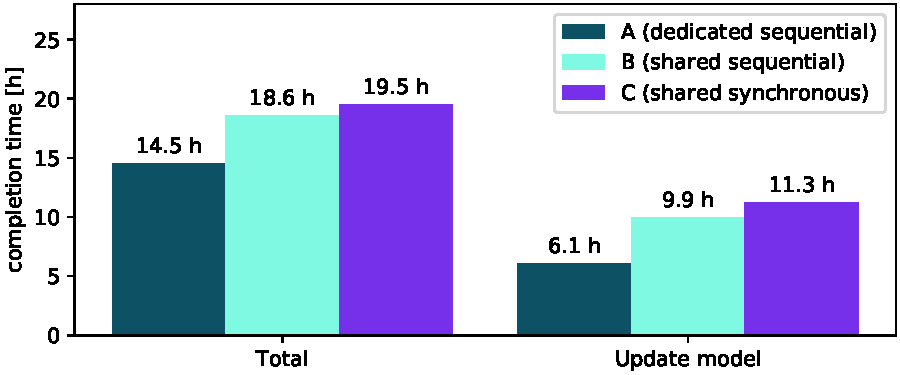
\includegraphics[width=\textwidth]{chart_interference_impact_completion}
		\subcaption{Completion time}\label{fig:chart-interference-impact-completion}
	\end{minipage}%
	\hfill
	\begin{minipage}[b]{.35\textwidth}
		\centering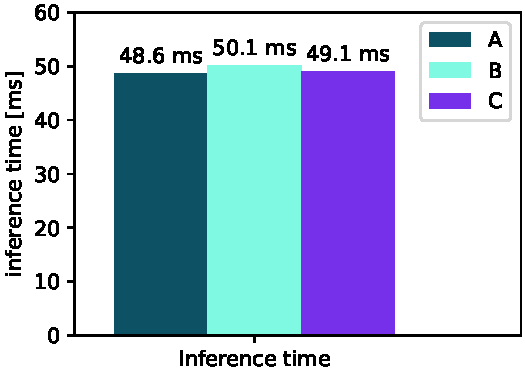
\includegraphics[width=\textwidth]{chart_interference_impact_inference}
		\subcaption{Inference performance}\label{fig:chart-interference-impact-inference}
	\end{minipage}
	\caption{Impact of interference}
	\label{fig:chart-interference-impact}
\end{figure}

We examine experiments D and E to evaluate the greedy and fair scheduler algorithm design, comparing them with A as baseline (Figure \ref{fig:chart-interleaving}). Using greedy interleaving, autotuning completes in \SI{20.4}{\hour}, \SI{5.9}{\hour} slower than A. While model update time stays about the same, \SI{5.5}{\hour} (27\%) of the total time is now spent waiting\footnote{Only stage execution times can be measured. Wait time and non-stage times (transfer learning, file operations) need to be derived. Non-stage times are about \SI{0.49}{\hour}, derived from A. Wait time for interleaving is calculated as follows: $t_{wait} = t_{total} - \sum_{i}t_{stage,i} - \SI{0.49}{\hour}$} for resources to become free to prevent interference. Fair interleaving is impacted even more by waiting, with total autotuning time increasing to \SI{24.1}{\hour}, \SI{9.6}{\hour} (+62\%) slower than A. Model update time remains about the same again, but wait time accumulates to \SI{8.9}{\hour} (37\% of total autotuning). Building and profiling time do not change for both. While the total completion time deteriorates, inference performance matches the baseline of \SI{48.6}{\milli\second} for both D and E.

\begin{figure}[t]
	\begin{minipage}[b]{.6\textwidth}
		\centering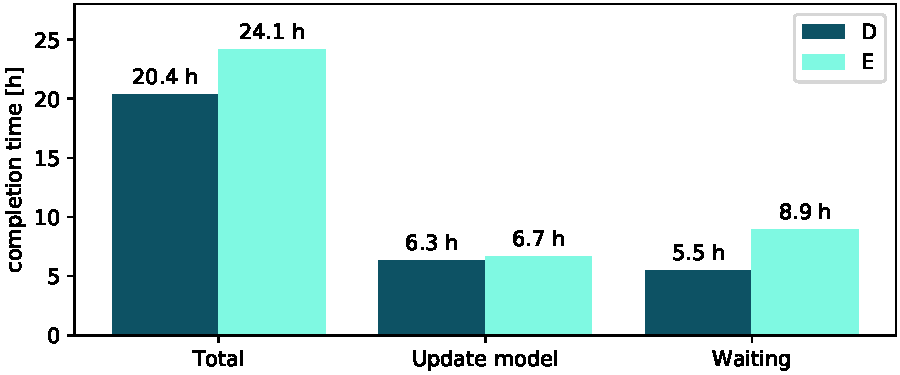
\includegraphics[width=\textwidth]{chart_interleaving_completion}
		\subcaption{Completion time}\label{fig:chart-interleaving-completion}
	\end{minipage}%
	\hfill
	\begin{minipage}[b]{.35\textwidth}
		\centering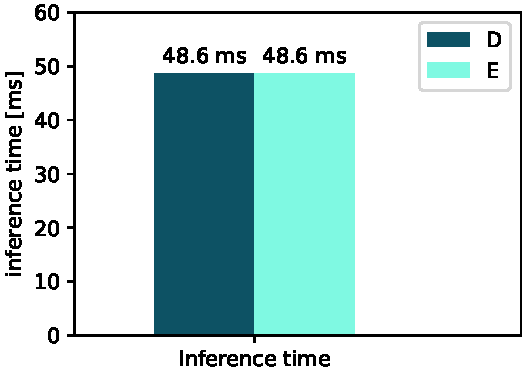
\includegraphics[width=\textwidth]{chart_interleaving_inference}
		\subcaption{Inference performance}\label{fig:chart-interleaving-inference}
	\end{minipage}
	\caption[Results of greedy versus fair interleaving]{Greedy versus fair interleaving}
	\label{fig:chart-interleaving}
\end{figure}

Finally, we examine the effect of employing stage bundling as opposed to individually scheduling them (Figure \ref{fig:chart-bundling}). The greedy algorithm is used in F, the fair algorithm is used in G. With bundling, greedy interleaving performs about the same as without bundling. On the other hand, fair interleaving completes \SI{2.4}{\hour} (-10\%) earlier than the individually scheduled version due to a total wait time that is \SI{2.7}{\hour} (-30\%) shorter. As before, model update time remains relatively similar. Inference time in F is \SI{0.4}{\milli\second} faster than in D, while G's is slower than E by \SI{0.3}{\milli\second}.

\begin{figure}[t]
	\begin{minipage}[b]{.6\textwidth}
		\centering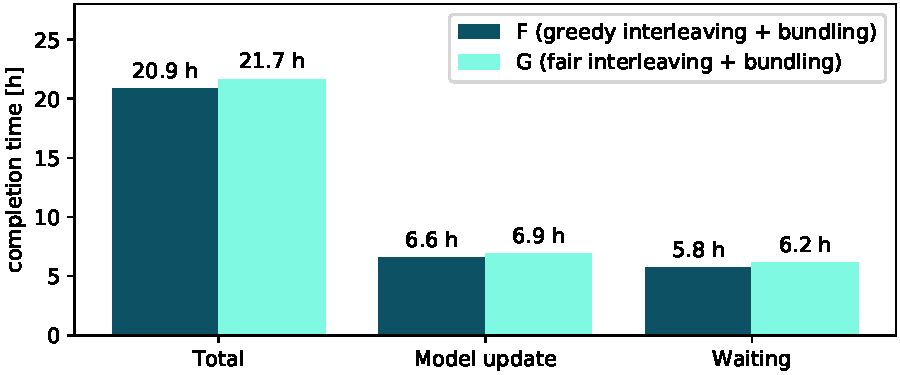
\includegraphics[width=\textwidth]{chart_bundling_completion}
		\subcaption{Completion time}\label{fig:chart-bundling-completion}
	\end{minipage}%
	\hfill
	\begin{minipage}[b]{.35\textwidth}
		\centering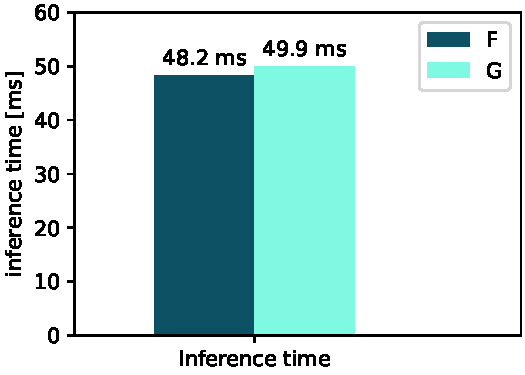
\includegraphics[width=\textwidth]{chart_bundling_inference}
		\subcaption{Inference performance}\label{fig:chart-bundling-inference}
	\end{minipage}
	\caption[Results of greedy versus fair interleaving with bundling]{Greedy versus fair interleaving with bundling}
	\label{fig:chart-bundling}
\end{figure}

\section{Discussion}
The objective of large-scale autotuning is to achieve the autotuning time and inference performance of running only a single job on each server, but with shared resources to keep the amount of required hardware at a minimum. Single-job autotuning is represented by Setup A, which is why we use it as baseline for comparisons with the other experiments. Because our evaluation is limited to a single machine type and model, more experiments are required for a general analysis.

In B and C we show the detrimental effects of interference on performance which motivated the creation of a scheduler. If it were not for this, resources could be shared and jobs could be run in parallel without control by a central entity. B and C behave relatively similar because even without explicit scheduling, both jobs run approximately synchronous since they autotune the same model. In real-world scenarios with diverse workloads, there might be a more drastic difference between B and C. The fact that C has faster inference than B is presumably caused by the probabilistic nature of configuration selection. The difference in inference performance of both to the baseline is relatively small due to the large number of trials which even out the impact of interference. However, even slightly worse inference speed has a large impact with an increasing number of inferences.

Note how interference is avoided with the scheduler in D--G, which manifests in stage times (particularly model updating) that are comparable to single-job autotuning as well as in a good inference performance. However, a significant amount of wait time is introduced which drives up total completion time. Greedy interleaving without bundling shows the shortest wait time in our experiments. Bundling does not show a big effect when comparing D and F because greedy interleaving naturally behaves like bundling. However, fair interleaving benefits much from bundling in our experiments, remedying the vast wait time.

Greedy interleaving works well in our experiments because both jobs are identical and the portion of time spent on the client machine versus time spent on the target device is roughly similar. As a result, wait time is reduced because, after an initial wait period, both jobs alternate nearly perfectly but mutually opposing between client and target. Despite these results, we believe that fair interleaving is the superior algorithm for scheduling heterogeneous jobs with varying complexity on a large scale, as would be the case with \gls{aaas}. Greedy interleaving would allow jobs to monopolize resources for an extended period of time, while fair interleaving allows for a finer control, especially if more resources are available. Bundling in conjunction with the fair algorithm is still an option to interleave homogeneous jobs on few resources, which would show the same effect as the greedy algorithm in our experiment.

Our scheduler is very rudimentary at this point, leaving much room for improvement. While the concept of interleaving seems promising, a more intelligent approach than fair round-robin could be employed to fill idle time optimally while keeping average wait time low. For example, a predictive scheduler could use knowledge from previous tasks to make a more educated decision that will maximize resource utilization. This would augment the notion of load-awareness with knowledge about the estimated stage execution time. Such a scheduler could then leverage the exact or heuristic interleaving algorithm from \cite{Ma.2005}. However, a more sophisticated algorithm might require finer control over the stages, which cannot be provided by the client's current resource/stage interface. Trading off a complex client but simple scheduler for a thin, stateless client and autotuning-aware scheduler by shifting responsibilities might become a necessity.

Furthermore, the scheduler needs to be enhanced with support for multiple resources of the same type. At this point, all target devices are regarded as a single, atomic resource. More granularity is essential for production-grade implementations in an \gls{aaas} platform. This would go hand in hand with eliminating the tracker and letting the scheduler assign target devices to clients. A trivial refinement is replacing the busy waiting for a stage to be done in the scheduler algorithm, resulting in an excess of redundant \gls{rpc} calls, by a push-based approach, where the client notifies the scheduler once a stage has completed.

We used our scheduler only for autotuning with TVM. However, other autotuning frameworks like \gls{tc} that have the same scaling issues might also profit from our solution. The \gls{aaas} platform might even provide support for a variety of autotuning frameworks.
	\chapter{Conclusion}
	Enabling large-scale autotuning is the foundation of any \gls{aaas} platform that uses our reference architecture. We demonstrated that our interleaving scheduler can leverage the fundamental weakness of resource idle time to make sharing of computation resources possible, which facilitates fast and economical autotuning while delivering good inference performance. This is a key step towards democratizing real-time \gls{dl} applications to power exciting innovations in a wide variety of fields.

Future efforts based on our work should focus on creating a more intelligent scheduler algorithm to improve the efficiency of multi-job autotuning. A resource provisioning algorithm will then complete the orchestrator component, paving the way for the development of a mature \gls{aaas} product.

	
	\clearpage
	
	%----------------------------------------------------------------------------
	% Appendix
	%----------------------------------------------------------------------------
	
	\cleardoublepage
	\printbibliography

	\printglossary[style=altlist]
	
	\clearpage
	\appendix
\end{document}